\documentclass[12pt, titlepage]{article}

\usepackage[dvipsnames]{xcolor} % for different colour comments
\usepackage{tabto}
\usepackage{mdframed}
\mdfsetup{nobreak=true}
\usepackage{xkeyval}
\usepackage{tabularx}
\usepackage{booktabs}
\usepackage{hyperref}
\hypersetup{
    colorlinks,
    citecolor=black,
    filecolor=black,
    linkcolor=red,
    urlcolor=blue
}
\usepackage[skip=2pt, labelfont=bf]{caption}
\usepackage{titlesec}
\usepackage{graphicx}
\graphicspath{ {image/} }



%% the following adds another section level by redefining the paragraph
%% source:  http://tex.stackexchange.com/questions/60209/how-to-add-an-extra-level-of-sections-with-headings-below-subsubsection
\setcounter{secnumdepth}{4}

\titleformat{\paragraph}
{\normalfont\normalsize\bfseries}{\theparagraph}{1em}{}
\titlespacing*{\paragraph}
{0pt}{3.25ex plus 1ex minus .2ex}{1.5ex plus .2ex}


%% Comments
\newif\ifcomments\commentstrue

\ifcomments
\newcommand{\authornote}[3]{\textcolor{#1}{[#3 ---#2]}}
\newcommand{\todo}[1]{\textcolor{red}{[TODO: #1]}}
\else
\newcommand{\authornote}[3]{}
\newcommand{\todo}[1]{}
\fi

\newcommand{\wss}[1]{\authornote{magenta}{SS}{#1}}
\newcommand{\ds}[1]{\authornote{blue}{DS}{#1}}



%% The following are used for pretty printing of events and requirements
\makeatletter

\define@cmdkey      [TP] {test}     {name}       {}
\define@cmdkey      [TP] {test}     {desc}       {}
\define@cmdkey      [TP] {test}     {type}       {}
\define@cmdkey      [TP] {test}     {init}       {}
\define@cmdkey      [TP] {test}     {input}      {}
\define@cmdkey      [TP] {test}     {output}     {}
\define@cmdkey      [TP] {test}     {pass}       {}
\define@cmdkey      [TP] {test}     {user}       {}
\define@cmdkey      [TP] {test}     {result}     {}


\newcommand{\getCurrentSectionNumber}{%
  \ifnum\c@section=0 %
  \thechapter
  \else
  \ifnum\c@subsection=0 %
  \thesection
  \else
  \ifnum\c@subsubsection=0 %
  \thesubsection
  \else
  \thesubsubsection
  \fi
  \fi
  \fi
}

\newcounter{TestNum}

\@addtoreset{TestNum}{section}
\@addtoreset{TestNum}{subsection}
\@addtoreset{TestNum}{subsubsection}

\newcommand{\testauto}[1]{
\setkeys[TP]{test}{#1}
\refstepcounter{TestNum}
\begin{mdframed}[linewidth=1pt]
\begin{tabularx}{\textwidth}{@{}p{3cm}X@{}}
{\bf Test \getCurrentSectionNumber.\theTestNum:} & {\bf \cmdTP@test@name}\\[\baselineskip]
{\bf Description:} & \cmdTP@test@desc\\[0.5\baselineskip]
{\bf Type:} & \cmdTP@test@type\\[0.5\baselineskip]
{\bf Initial State:} & \cmdTP@test@init\\[0.5\baselineskip]
{\bf Input:} & \cmdTP@test@input\\[0.5\baselineskip]
{\bf Output:} & \cmdTP@test@output\\[0.5\baselineskip]
{\bf Expected:} & \cmdTP@test@pass\\[\baselineskip]
{\bf Result:} & \cmdTP@test@result
\end{tabularx}
\end{mdframed}
}

\newcommand{\testautob}[1]{
\setkeys[TP]{test}{#1}
\refstepcounter{TestNum}
\begin{mdframed}[linewidth=1pt]
\begin{tabularx}{\textwidth}{@{}p{3cm}X@{}}
{\bf Test \getCurrentSectionNumber.\theTestNum:} & {\bf \cmdTP@test@name}\\[\baselineskip]
{\bf Description:} & \cmdTP@test@desc\\[0.5\baselineskip]
{\bf Type:} & \cmdTP@test@type\\[0.5\baselineskip]
{\bf Pass:} & \cmdTP@test@pass
\end{tabularx}
\end{mdframed}
}

\newcommand{\testmanual}[1]{
\setkeys[TP]{test}{#1}
\refstepcounter{TestNum}
\begin{mdframed}[linewidth=1pt]
\begin{tabularx}{\textwidth}{@{}p{3cm}X@{}}
{\bf Test \getCurrentSectionNumber.\theTestNum:} & {\bf \cmdTP@test@name}\\[\baselineskip]
{\bf Description:} & \cmdTP@test@desc\\[0.5\baselineskip]
{\bf Type:} & \cmdTP@test@type\\[0.5\baselineskip]
{\bf Tester(s):} & \cmdTP@test@user\\[0.5\baselineskip]
{\bf Pass:} & \cmdTP@test@pass
\end{tabularx}
\end{mdframed}
}


\makeatother

\newcommand{\ZtoT}{
\begin{tabularx}{3.85cm}{@{}p{0.35cm}p{0.35cm}p{0.35cm}p{0.35cm}p{0.35cm}p{0.35cm}p{0.35cm}p{0.35cm}p{0.35cm}p{0.35cm}p{0.35cm}@{}}
0 & 1 & 2 & 3 & 4 & 5 & 6 & 7 & 8 & 9 & 10
\end{tabularx}
}

\begin{document}
\title{\bf Platform Perils\\[\baselineskip]\Large Test Report}
\author{Steven Palmer\\$\langle$palmes4$\rangle$\\Chao Ye\\$\langle$yec6$\rangle$}
\date{\today}
	
\maketitle

\pagenumbering{roman}
\tableofcontents
\listoftables
\listoffigures


\begin{table}[bp]
\caption*{\bf Revision History}
\begin{tabularx}{\textwidth}{p{3.5cm}p{2cm}X}
\toprule {\bf Date} & {\bf Version} & {\bf Notes}\\
\midrule
March 24, 2016 & 1.0 & Created document skeleton\\
March 28, 2016 & 1.1 & Final version for rev 0\\
\bottomrule
\end{tabularx}
\end{table}

\newpage

\pagenumbering{arabic}


\section{Introduction}

This document provides a report of the results of the testing performed on the Platform Perils application.  Both system testing and quality testing are covered. Traceability between testing and both requirements and modules is given in the final section.


\section{System Testing}

\noindent**{\bf NOTE 1:}  Many of the automated tests described in the test plan will not be implemented in this version of the game.  The test plan will be modified for revision 1 submission to achieve consistency. **\\[10pt]
\noindent**{\bf NOTE 2:}  Additional automated testing is planned for revision 1.**



\subsection{Automated Testing}

A suite of automated unit tests has been created to test the game for basic functionality.  The unit tests cover input response as well as collision physics.  These tests are useful to ensure that modifications to the game code do not break the fundamentals of the game.  A description of the unit tests that were carried out and their results are given in the remainder of this section.

\testauto{
    name = {Walk left, started from stationary},
    desc = Tests if the hero walks left when the corresponding input is received when the hero is initially stationary,
    type = {Unit Test (dynamic, automated)},
    init = Custom in-game state with a hero object having x-velocity of zero,
    input = Keyboard function called with simulated left key down stroke,
    output = Hero object x-velocity,
    pass = Hero object x-velocity is less than zero,
    result = \textcolor{Green}{PASS}
}

\testauto{
    name = {Walk right, started from stationary},
    desc = Tests if the hero walks right when the corresponding input is received when the hero is initially stationary,
    type = {Unit Test (dynamic, automated)},
    init = Custom in-game state with a hero object having x-velocity of zero,
    input = Keyboard function called with simulated right key down stroke,
    output = Hero object x-velocity,
    pass = Hero object x-velocity is greater than zero,
    result = \textcolor{Green}{PASS}
}

\testauto{
    name = {Supported by platform},
    desc = Tests if the hero is supported when standing on a platform,
    type = {Unit Test (dynamic, automated)},
    init = Custom in-game state with a hero object having zero velocity directly above a platform,
    input = The game is stepped forward in time,
    output = Hero object y-position,
    pass = Hero object y-position is unchanged,
    result = \textcolor{Green}{PASS}
}

\testauto{
    name = {Obstructed by wall, approaching from left side},
    desc = Tests if the hero is obstructed by a wall when approaching from the left side of the wall,
    type = {Unit Test (dynamic, automated)},
    init = Custom in-game state with a hero object on a platform with a wall directly to the right,
    input = Keyboard function called with simulated right key down stroke and the game is stepped forward in time,
    output = Hero object x-position,
    pass = Hero object x-position is unchanged,
    result = \textcolor{Green}{PASS}
}

\testauto{
    name = {Obstructed by wall, approaching from right side},
    desc = Tests if the hero is obstructed by a wall when approaching from the right side of the wall,
    type = {Unit Test (dynamic, automated)},
    init = Custom in-game state with a hero object on a platform with a wall directly to the left,
    input = Keyboard function called with simulated left key down stroke and the game is stepped forward in time,
    output = Hero object x-position,
    pass = Hero object x-position is unchanged,
    result = \textcolor{Green}{PASS}
}


\subsection{Manual Testing}

Manual testing was the main method used to ensure that the game functions as intended.  A summary of the results of the manual testing are given in \hyperref[tab:man]{Table~\ref*{tab:man}}.

\begin{table}[ht]
\caption{Manual test results} \label{tab:man}
\begin{tabularx}{\textwidth}{p{5cm}X}
\toprule {\bf Test category} & {\bf Result}\\
\midrule
Gameplay & \textcolor{Green}{PASS}\\
Sound & \textcolor{Green}{PASS}\\
Graphics & Texture problem on arch needs fixing.\\
\bottomrule
\end{tabularx}
\end{table}



\section{Quality Testing}

\subsection{Usability Testing}
A user experience survey will be used to assess useability.  This survey has not yet been administered but is expected to occur in the near future.

\subsection{Performance Testing}
Stress testing was used to evaluate performance.  In these tests, different types of game objects were continuously introduced to a stage while measuring changes in framerate.  A high performance and low performance system were used in these tests.  The specifications of each system is given in \hyperref[tab:systems]{Table~\ref*{tab:systems}}.

\begin{table}[ht]
\caption{Systems used in performance testing} \label{tab:systems}
\begin{tabularx}{\textwidth}{p{5cm}X}
\toprule {\bf System} & {\bf Hardware}\\
\midrule
High performance & i7 4770K @ 4.4 GHz\\
& AMD Radeon HD 7970\\[10pt]
Low performance & i5 2430M @ 2.4 GHz\\
& nVidia GT 540M\\
\bottomrule
\end{tabularx}
\end{table}

The objects used by the game can be broken down into two main categories:  dynamic and static.  Dynamic objects are free moving and subject to all physics calculations, while static objects do not move and are only involved in collision calculations.  All dynamic objects used in the game are essentially the same: they consist of a loaded mesh, textures, and a single shader.  Most static objects also fit this description, with one notable exception:  platform objects were implemented using 3 separate shaders.

Plots showing the variation in framerate with respect to the number of objects present in a stage are given in \hyperref[fig:frdynamic]{Figure~\ref*{fig:frdynamic}} (dynamic) and \hyperref[fig:frstat]{Figure~\ref*{fig:frstat}} (static).  The results show that a large number of objects can be incorporated into a stage before performance begins to be affected:  the high performance system maintained a framerate of 60 fps until roughly 1500 dynamic objects or 3000 static objects were introduced.  Even the low performance system was able to maintain a framerate above 60 until around 300 dynamics objects.  This means that the game will likely be able to run at 60 fps on most systems since the number of objects in a single stage is unlikely to approach 300.  

A plot showing the variation in framerate with respect to the number of platforms was also produced and is shown in \hyperref[fig:frplat]{Figure~\ref*{fig:frplat}}.  The results of this test show a drastic drop in framerate with very few objects, and this framerate drop appears to be consistent between the high end and low end systems.  This suggests that the problem is in using multiple shaders:  switching shaders is a resource intensive procedure and the consistencies in framerate between the two systems can be explained by the fact that the amount of time required for switching a shader would be approximately constant between the two systems.

\begin{figure}[H]
\centering
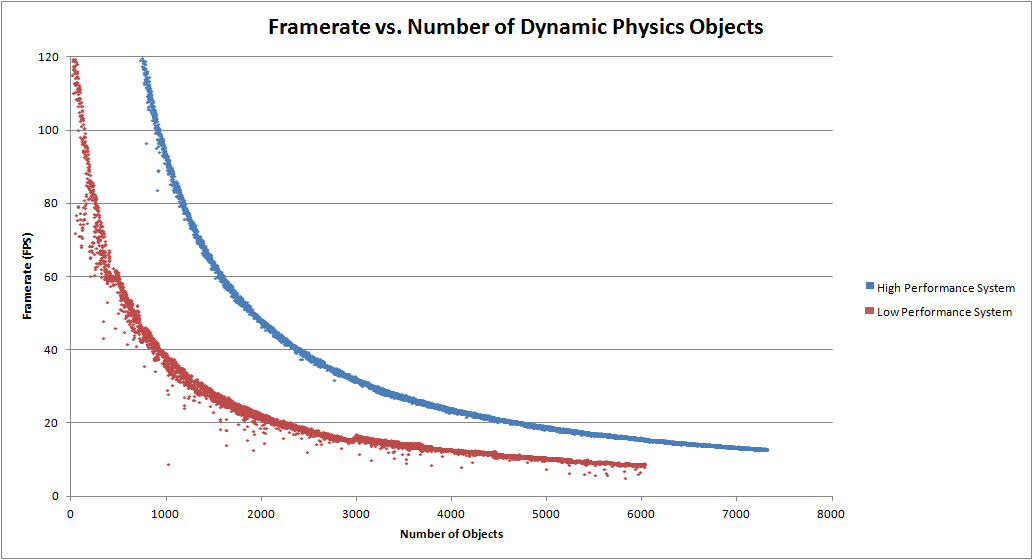
\includegraphics[width=\textwidth]{frameratedynamic}
\caption{Framerate vs. number of dynamic objects} \label{fig:frdynamic}
\end{figure}


\begin{figure}[H]
\centering
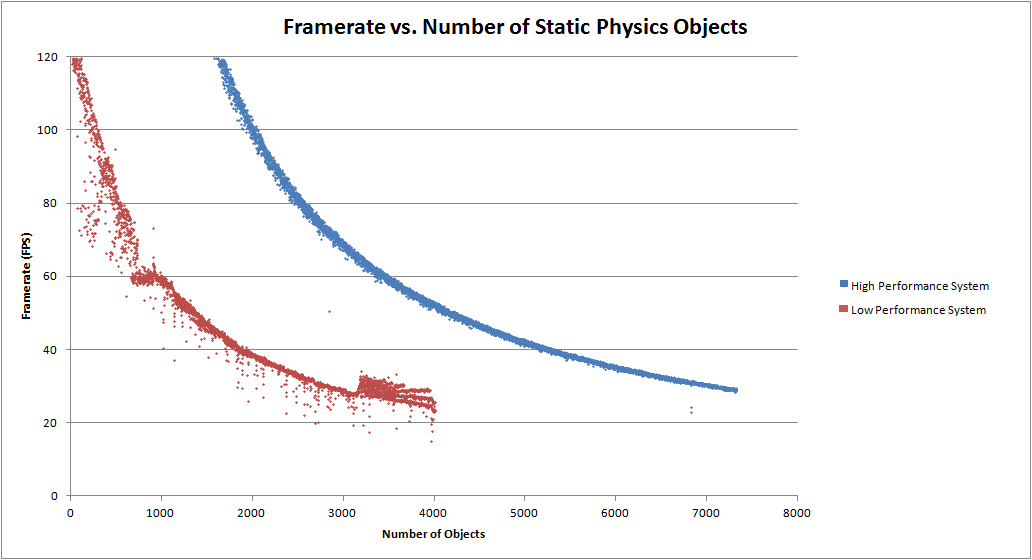
\includegraphics[width=\textwidth]{frameratestatic}
\caption{Framerate vs. number of static objects} \label{fig:frstat}
\end{figure}

\begin{figure}[H]
\centering
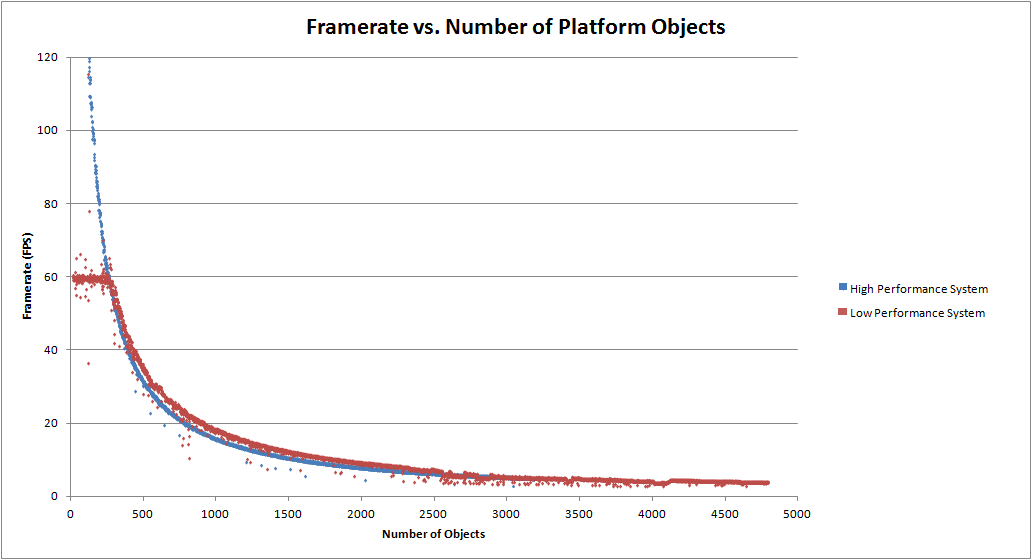
\includegraphics[width=\textwidth]{framerateplat}
\caption{Framerate vs. number of platform objects} \label{fig:frplat}
\end{figure}

\begin{figure}[H]
\centering
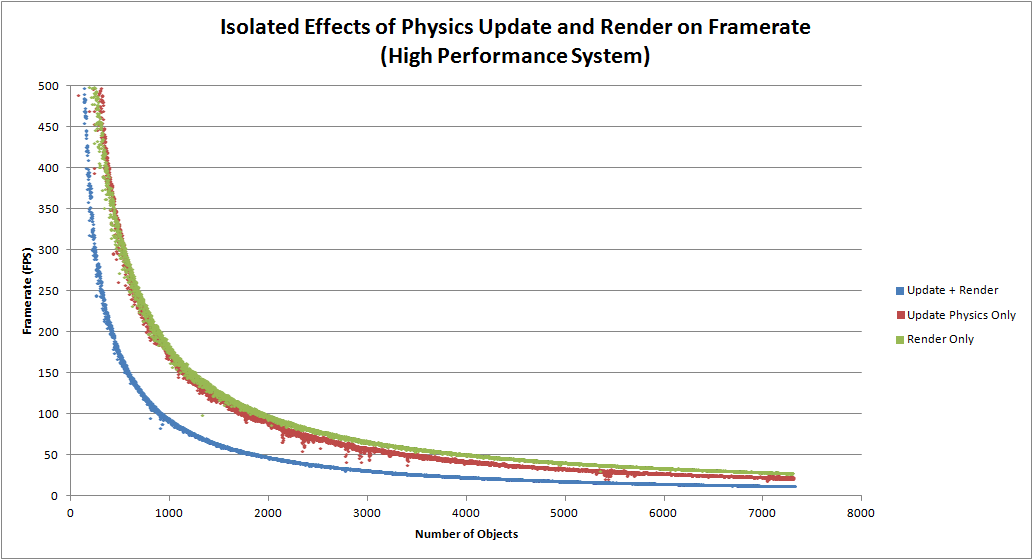
\includegraphics[width=\textwidth]{isolatedhigh}
\caption{Effects of physics update and render on framerate on high performance system} \label{fig:isohi}
\end{figure}


\begin{figure}[H]
\centering
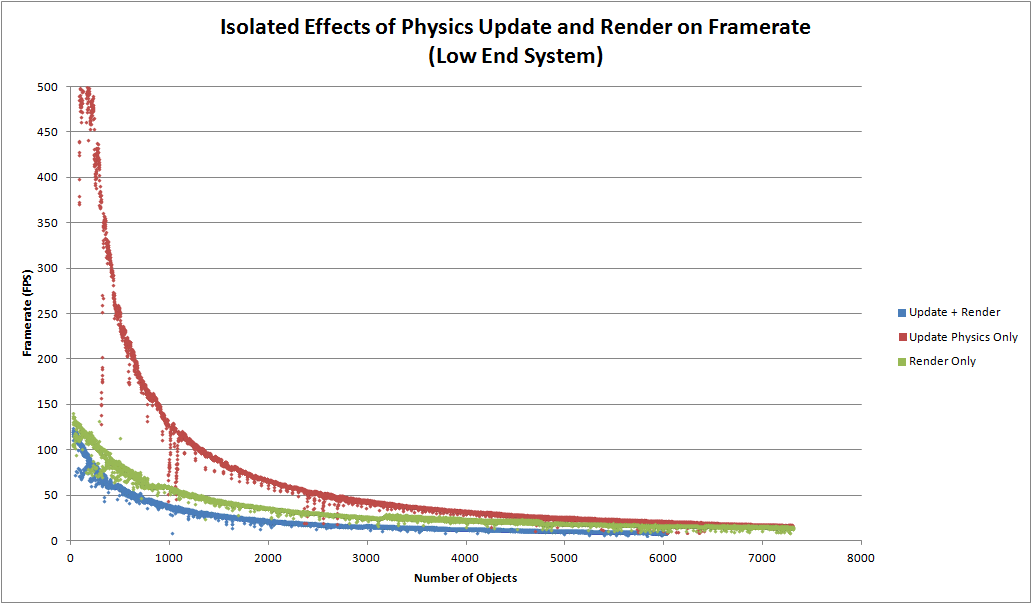
\includegraphics[width=\textwidth]{isolatedlo}
\caption{Effects of physics update and render on framerate on low performance system} \label{fig:isolo}
\end{figure}

Additional testing was performed to assess whether the framerate was predominantly affected by procedures involving physics calculations or rendering.  The results of these tests are given in \hyperref[fig:isohi]{Figure~\ref*{fig:isohi}} and \hyperref[fig:isolo]{Figure~\ref*{fig:isolo}} for the high and low performance systems, respectively.  Interestingly, from the plot of the high performance system it appears that neither is a dominant factor:  both make a roughly equal contribution to the overall framerate.  This does not appear to be the case in the low performance system, where it is clear that the rendering step limits the framerate.  



\subsection{Robustness Testing}
Robustness of the application with regard to erroneous input was not formally tested.  User inputs are only accepted as defined keystrokes and mouse clicks.  The way these inputs map to setting/modifying variables is entirely controlled by the game code and thus the user is never able to directly change any variables via inputs.  This means that all variables are maintained within their expected ranges and no explicit testing is required.

Robustness tests in the form of stress testing were covered under performance testing.

\section{Summary of Changes}
A summary of the changes made in response to testing are given in \hyperref[tab:changes]{Table~\ref*{tab:changes}}.\\

\noindent** {\bf Note:} Changes have not yet been made. **

\begin{table}[ht]
\caption{Changes made in response to testing} \label{tab:changes}
\begin{tabularx}{\textwidth}{p{5cm}X}
\toprule {\bf System} & {\bf Hardware}\\
\midrule
\\
\bottomrule
\end{tabularx}
\end{table}

\section{Traceability}
\subsection{Trace of Testing to Requirements}
A trace between requirements and testing is given in \hyperref[tab:tracereq]{Table~\ref*{tab:tracereq}}.\\

\noindent** {\bf NOTE:}  Requirements need updating.  This will be done before revision 1. **

\begin{table}[ht]
\caption{Trace between requirements and tests} \label{tab:tracereq}
\begin{tabularx}{\textwidth}{p{5cm}X}
\toprule {\bf Requirement} & {\bf Test(s)}\\
\midrule
&\\
\bottomrule
\end{tabularx}
\end{table}
\subsection{Trace of Testing to Modules}
A trace between modules and testing is given in \hyperref[tab:tracemod]{Table~\ref*{tab:tracemod}}.\\

\noindent** {\bf NOTE:} The design document needs updating.  This will be done before revision 1. **
\begin{table}[ht]
\caption{Trace between modules and tests} \label{tab:tracemod}
\begin{tabularx}{\textwidth}{p{5cm}X}
\toprule {\bf Module} & {\bf Test(s)}\\
\midrule
&\\
\bottomrule
\end{tabularx}
\end{table}



\end{document}
